\chapter{Application Prototype}
\label{ch:Prototype}
Before making a start on of the implementation phase, a lot of effort was put into the creation of the application prototype. Prototyping is a process of developing the initial model of the future application in order to determine the correct application structure, its functionality and the general concept. A prototype is just a model and may differ from the final product.

The project requirements outlined in the previous chapter of this report were used in order to create a mind map representing pages of the future application. This helped understanding what exactly is expected to be seen on each page of the website and what is the user journey in terms of the navigation. Wireframes were created for all the pages of the website. For this purpose was used just paper and pencils to aim flexibility.

In terms of the methodology, a hybrid of Agile and the traditional Waterfall approach was used for this project. Speaking of the traditional Waterfall approach, some of planning was made beforehands, for example requirements specifications, use-case diagrams, wireframes, etc. On the other hand, for the whole implementation phase was used test-driven approach that utilises the best of the agile techniques.

In general, Agile methodology focuses on team communication and project transparency. Nevertheless, one of its advantages is an extreme flexibility, therefore most of the basic components of Agile can still be effectively used by a single person. The key feature of the version of Agile adopted for the project was breaking down the project workload into clearly defined units of work (high-level features introduced in the chapter "Requirements Analysis" \ref{ch:requirementanalysis}), each associated with an iteration, and setting a milestone for each of them. Excel sheets were used for defining the set of tasks for each iteration. GitHub issue tracker was also used as a supporting productivity tool for this project. Code related tasks were recorded as "issues" for the project GitHub repository. The GitHub issue tracker appeared to be a very efficient tool for keeping the focus. TDD or test driven develoment was another key Agile technique adopted for the project. The unit tests covering business logic were always written before the implementation and the next sprint has not been started unless all tests from the previous sprint passed. 

In summary, in this section will be described the process of transforming project requirements into the system design. Several design cornerstones (website structure mind map, a set of wireframes, usecases) were produced beforehands. Other elements of the application design (database schema) were updated in iterations, inline with the Agile methodology. 

\section{Application Structure}
\label{sec:applicationstructure_prototype}
The prototyping process started with producing a large mind map of the future application. I found mindmapping a very useful way to brainstorm on my ideas, capture and organise them. The final version of the diagram puts together the structure of application pages, navigation scenarios and other ideas relevant to the design. A part of the developed mind map can be found in the figure below.

\begin{figure}[H]
	\begin{center}
		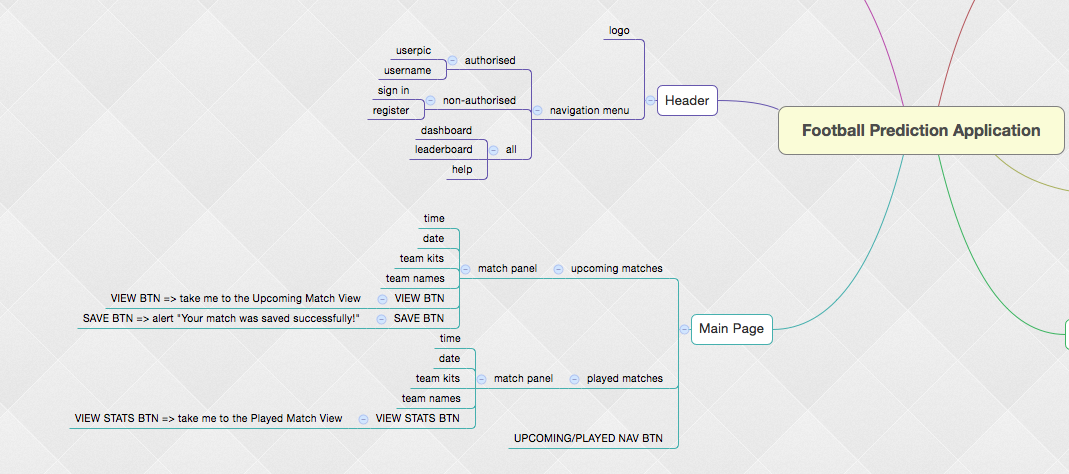
\includegraphics[width=.90\textwidth]{design/images/mindmap}
		\caption{Mind map capturing the result of the initial brainstorming on the application structure and navigation scenarios.}
		\label{fig:using:mindmap}
	\end{center}
\end{figure}

\section{Analysis of the competitors experience}
\label{sec:competitors_prototype}
As the next step, I took another look at the existing websites, expecting to get some ideas on how to approach the visual side of the project and to improve its usability. This step is an important stage of an application prototyping process: it allows to learn from the best design practices and possibly avoid potential errors. The usual practice is to first concentrate on few websites of the direct competition. However, it was not possible to identify the direct competitors, as the idea behind the project is quite unique. Therefore, I analysed several football statistics and community websites, namely \emph{WhoScored?} \citep{source:whoscored}, \emph{Goal.com} \citep{source:goal} and \emph{OLGB Betting Community} \citep{source:olgb}, making a note of how those websites present football statistics to their users, what are the main differences between the presentation of an unplayed and played match, what interesting features each website offer to its audience. This analysis served as a great source of inspiration and the basis for the next step - producing the wireframes.

\section{Wireframes}
\label{sec:wireframes_prototype}
When speaking about prototyping, in the early stages the first choice of many designers is often a piece of paper and a pencil. Sketching has a number of advantages when compared to the use of the graphic design software, such as Fireworks or Photoshop. When using the editors, it is easy to get distracted by brushing up unnecessary details too early. On the opposite side, sketches offer a lot of flexibility. It is easy to add notes, make small changes or replace an outdated sketch with a fresh one.

In case of this project, each of the sketches represented a separate “view” of the website. The scale of a “view” might differ. For example, some sketches show a whole page (home page, dashboard page, etc.), others only capture a part of a page (a header, a footer, user profile menu) in more detail.  Below can be found scans of the project wireframes.

Scans of the drawings

\section{Visual Design.}
\label{sec:visdesign_prototype}
At this stage of the prototyping process I started thinking of choosing a suitable name for the future application. Below is the list of some names that were considered at this stage.

\begin{itemize}
	\item Too Close To Call
	\item Sure Thing
	\item Footy Expert
	\item Shortening the Odds
\end{itemize}

\emph{SureThing} was chosen as the project name for being unique, simple and catchy, while expressing the essence of the future application. The name evokes optimistic feelings and is quite suitable for a prediction system that is transparent to its users and will increase their chances to win a bet in the long run. 

As it can be seen from the long list of the mandatory requirements, the project will require a lot of time to be invested in implementing the functionality. Therefore, it was decided to make use of Twitter Bootstrap framework on the front end \citep{documentation:Bootstrap3} \citep{web:templateProgressus} in order to reduce the amount of time spent developing the visual side of the application and create simple and consistent interface. As a result, the final design is a mixture of Bootsrap snippets and my own ideas on how to visualize unique elements of the application layout, such as dashboard side menu, match panels in matches overview, prediction modules layout in upcoming match view and many others. 

\section{Use Cases}
\label{usecases_prototype}
As mentioned above, use cases and the database scheme presented below, were developed in iterations. In this report will be presented a completed, merged version of the set of the use cases and the database design diagram. 

This section will concentrate on the use cases - the graphical illustration of the system functionality. UML will be used to design in a clear and readable manner. 

As a User I would like to view the most popular blu-ray discs sold


\begin{figure}[H]
	\begin{center}
		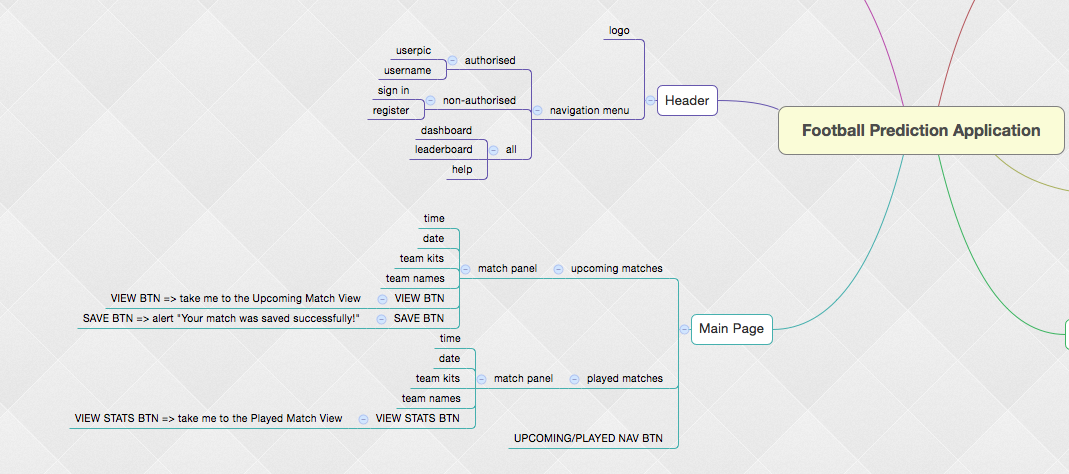
\includegraphics[width=.90\textwidth]{design/images/mindmap}
		\caption{This use case diagram shows the typical sequence of steps a user will take when saving a match to the dashboard.} \label{fig:using:usecase1}
	\end{center}
\end{figure}
This Diagram shows the typical activities a user will complete when using the shared expense area of the application, and how the activities the system will need to complete as a result of some user actions

\section{Database Schema}
\label{databaseschema_prototype}
The application makes use of a database and a database schema holds together the group of entities or models used by the application. As already mentioned above, the schema for this project was developed in an iterative way along with the development of the high level features of the application: the tables and relationships between them were added gradually. The final version of the diagram is a result of numerous iteration and can be found below.


what database was used
Use this link to describe the ORM and its advantages: 
http://www.aosabook.org/en/sqlalchemy.html

